\documentclass[UTF8]{ctexart}

% 页面设置
\usepackage[a4paper]{geometry}
% 一般数学公式
\usepackage{amssymb}
\usepackage{amsmath}
% 有关数学模式西里尔字母 э 引用（详见 Commands）
\usepackage[T2A,T1]{fontenc}
% 图片引用
\usepackage{graphicx}
% 子图引用
\usepackage{subfig}
% 引用高亮
\usepackage[backref]{hyperref}
% 化学方程式包（用于打CO2）
\usepackage{chemformula}
% 国际单位制包（用于打带单位数值）
\usepackage{siunitx}
% 浮动体控制
\usepackage{float}
% toprule、midrule、bottomrule
\usepackage{booktabs}

\usepackage{tikz}
\usetikzlibrary{
	calc,
	positioning,
	patterns,
	arrows.meta,
	positioning,
	shapes.geometric,
	fit,
	decorations.pathmorphing
}


\newcommand{\rmd}{\mathrm{d}}

\title{公式推导}
\author{贺子旭}
\date{\today}
\begin{document}
	\maketitle
	\tableofcontents
	\newpage
	% 正文
	\setcounter{page}{1}
	\section{两球三弹簧谐振子}
		如图\ref{fig:2-balls-3-strings}，
		该物理模型由两个完全相同的小球（质量为$m$）
		与三个弹簧（劲度系数$k = m \omega^2$）连接，
		以及两面质量无穷大的刚体墙构成。
		\begin{figure}[H]
			\centering
			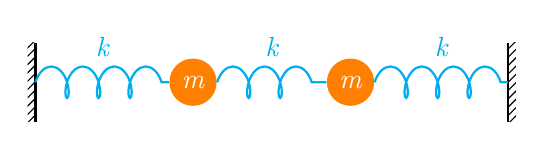
\begin{tikzpicture}[
				wall/.style={thick},
				spring/.style={thick, cyan, decoration={coil, segment length=0.4cm, amplitude=0.2cm}, decorate},
				mass/.style={circle, fill=orange, text=white, font=\itshape, inner sep=0pt, minimum size=0.6cm}
			]
				% 绘制墙
				\draw[wall] (0, -0.5) -- (0, 0.5);
				\fill[pattern=north east lines] (0, -0.5) rectangle (-0.1, 0.5);
				\draw[wall] (6, -0.5) -- (6, 0.5);
				\fill[pattern=north east lines] (6, -0.5) rectangle (6.1, 0.5);
				% 质量球
				\node[mass] (leftmass)   at (2,0) {\itshape m};
				\node[mass] (rightmass)  at (4,0) {\itshape m};
				% 节点
				\coordinate (left-wall)          at (0, 0);
				\coordinate (left-mass-left)     at $(leftmass.west);
				\coordinate (left-mass-right)    at $(leftmass.east);
				\coordinate (right-mass-left)    at $(rightmass.west);
				\coordinate (right-mass-right)   at $(rightmass.east);
				\coordinate (right-wall)         at (6, 0);
				% 绘制弹簧
				\draw[spring] (left-wall)        -- (left-mass-left)  node[midway, above=0.2cm] {\itshape k};
				\draw[spring] (left-mass-right)  -- (right-mass-left) node[midway, above=0.2cm] {\itshape k};
				\draw[spring] (right-mass-right) -- (right-wall)      node[midway, above=0.2cm] {\itshape k};
			\end{tikzpicture}
			\caption{两球三弹簧谐振子}
			\label{fig:2-balls-3-strings}
		\end{figure}

		该系统的拉格朗日量如下表示。
		\begin{equation}
			\begin{cases}
				L = T - V                                                                                                                          \\
				T = \dfrac{1}{2} m \dot{x}_{1}^{2} + \dfrac{1}{2} m \dot{x}_{2}^{2}                                                                  \\
				V = \dfrac{1}{2} m \omega^2 x_{1}^{2} + \dfrac{1}{2} m \omega^2 x_{2}^{2} + \dfrac{1}{2} m \omega^2 \left(x_{1} - x_{2}\right)^{2}    \\
			\end{cases}
		\end{equation}
		
		此时有
		\begin{equation}
			\begin{cases}
				\dfrac{\partial}{\partial x_1}L - \dfrac{d}{dt}\left(\dfrac{\partial}{\partial \dot{x}_{1}}L\right) = 0 \\
				\dfrac{\partial}{\partial x_2}L - \dfrac{d}{dt}\left(\dfrac{\partial}{\partial \dot{x}_{2}}L\right) = 0 \\
			\end{cases}
			\Longrightarrow
			\dfrac{\rmd^{2}}{{\rmd t}^{2}}
			\left(
				\begin{matrix}
					x_{1} \\
					x_{2} \\
				\end{matrix}
			\right)
			+
			\omega^2
			\left[
				\begin{matrix}
					2 & -1 \\
					-1 & 2 \\
				\end{matrix}
			\right]
			\left(
				\begin{matrix}
					x_{1} \\
					x_{2} \\
				\end{matrix}
			\right)
			= 0
			\label{eq:2-balls-3-strings-Lx2}
		\end{equation}

		对角化即有
		\begin{equation}
			\dfrac{\rmd^{2}}{{\rmd t}^{2}}
			\left(
				\begin{matrix}
					\dfrac{1}{\sqrt{2}} \left(x_{1} + x_{2}\right) \\
					\dfrac{1}{\sqrt{2}} \left(x_{1} - x_{2}\right) \\
				\end{matrix}
			\right)
			+
			\omega^2
			\left[
				\begin{matrix}
					1 & 0 \\
					0 & 3 \\
				\end{matrix}
			\right]
			\left(
				\begin{matrix}
					\dfrac{1}{\sqrt{2}} \left(x_{1} + x_{2}\right) \\
					\dfrac{1}{\sqrt{2}} \left(x_{1} - x_{2}\right) \\
				\end{matrix}
			\right)
			= 0
		\end{equation}

		即有
		\begin{gather}
			x_{1} + x_{2} = C_{\mathrm{c1}} \cos (         \omega t) + C_{\mathrm{s1}} \sin (         \omega t) \\
			x_{1} - x_{2} = C_{\mathrm{c3}} \cos (\sqrt{3} \omega t) + C_{\mathrm{s3}} \sin (\sqrt{3} \omega t)
		\end{gather}

		其中$C_{\mathrm{c1}}$、$C_{\mathrm{s1}}$、$C_{\mathrm{c3}}$、$C_{\mathrm{s3}}$均为与初始状态相匹配的常数。
		
		初始状态与常数的关系如下
		\begin{equation}
			\begin{cases}
				x_{1}      (t = 0) = X_{1} \\
				x_{2}      (t = 0) = X_{2} \\
				\dot{x}_{1}(t = 0) = V_{1} \\
				\dot{x}_{2}(t = 0) = V_{2} \\
			\end{cases}
			\Longrightarrow
			\begin{cases}
				C_{\mathrm{c1}} =       X_{1} + X_{2}            \\
				C_{\mathrm{c3}} =       X_{1} - X_{2}            \\
				C_{\mathrm{c1}} = \dfrac{V_{1} + V_{2}}{         \omega} \\
				C_{\mathrm{c3}} = \dfrac{V_{1} - V_{2}}{\sqrt{3} \omega} \\
			\end{cases}
		\end{equation}
	\newpage

	\section{双摆系统}
		如图\ref{fig:double-pendulum}，两个完全相同的小球通过长度相同的不可延伸硬杆相连接，构成双摆。
		该系统具备混沌的特点，但并非所有初态均对应混沌状态。
		\begin{figure}[H]
			\centering
			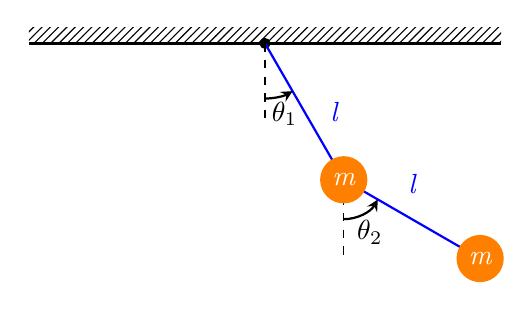
\begin{tikzpicture}[
				wall/.style={thick},
				string/.style={thick, blue},
				mass/.style={circle, fill=orange, text=white, font=\itshape, inner sep=0pt, minimum size=0.6cm},
				angle/.style={->, >=stealth, thick}
			]
				% 墙
				\draw[wall]   (-3,  0)     -- (3,      0);
				\fill[pattern=north east lines] (-3,0) rectangle (3,0.2);
				% 坐标
				\coordinate (loc0) at (0, 0);
				\coordinate (loc1) at (   1, -1.732);
				\coordinate (loc2) at (2.732,-2.732);

				% 支点
				\fill (loc0) circle (2pt);

				% 细线
				\draw[string] (loc0) -- (loc1) node[midway, right=0.2cm] {\itshape l};
				\draw[string] (loc1) -- (loc2) node[midway, above=0.2cm] {\itshape l};
				
				% 参考垂线
				\draw[dashed] (loc0) -- (0, -1);
				\draw[dashed] (loc1) -- ($(loc1) + (0, -1)$);

				% 角度标志线
				\draw[angle] (loc0) ++ (0,-0.7) arc (270: 300: 0.7);
				\draw[angle] (loc1) ++ (0,-0.5) arc (270: 330: 0.5);

				% 角度
				\node at (0.25, -0.9) {$\theta_1$};
				\node at (1.33, -2.4) {$\theta_2$};

				% 质量球
				\node[mass] (ball1)  at (loc1) {\itshape m};
				\node[mass] (ball2)  at (loc2) {\itshape m};
			\end{tikzpicture}
			\caption{双摆系统}
			\label{fig:double-pendulum}
		\end{figure}

		\subsection{物理过程}
			该体系拉格朗日量如下所示
			\begin{equation}
				\begin{cases}
					L = T - V                                                                                                                         \\
					T = \dfrac{1}{2} m \dot{x}_{1}^{2} + \dfrac{1}{2} m \dot{x}_{2}^{2} + \dfrac{1}{2} m \dot{y}_{1}^{2} + \dfrac{1}{2} m \dot{y}_{2}^{2} \\
					V = -m g y_{1} - m g y_{2}
				\end{cases}
			\end{equation}
			根据双摆的规则，有
			\begin{equation}
				\begin{cases}
					x_{1} = l \sin(\theta_1)                         \\
					x_{2} = l \sin(\theta_1) + l \sin(\theta_2)      \\
					y_{1} = l \cos(\theta_1)                         \\
					y_{2} = l \cos(\theta_1) + l \cos(\theta_2)      \\
				\end{cases}
				\Longrightarrow
				\begin{cases}
					\dot{x}_{1} =  l \cos(\theta_1) \dot{\theta}_1                                        \\
					\dot{x}_{2} =  l \cos(\theta_1) \dot{\theta}_1 + l \cos(\theta_2) \dot{\theta}_2      \\
					\dot{y}_{1} = -l \sin(\theta_1) \dot{\theta}_1                                        \\
					\dot{y}_{2} = -l \sin(\theta_1) \dot{\theta}_1 - l \sin(\theta_2) \dot{\theta}_2      \\
				\end{cases}
			\end{equation}

			代入则有
			\begin{equation}
				\begin{cases}
					T = \dfrac{1}{2} m l^2 \left(\cos^2(\theta_1) \dot{\theta}_{1}^{2} + \left(\cos(\theta_1) \dot{\theta}_1 + \cos(\theta_2) \dot{\theta}_2\right)^{2} + \sin^2(\theta_1) \dot{\theta}_{1}^{2} + \left(\sin(\theta_1) \dot{\theta}_1 + \sin(\theta_2) \dot{\theta}_2\right)^2\right) \\
					V = -2 m g l \cos(\theta_1) - m g l\cos(\theta_2)
				\end{cases}
			\end{equation}

			即
			\begin{gather}
				\begin{cases}
					T = \dfrac{1}{2} m l^2 \left(2 \dot{\theta}_{1}^{2} + \dot{\theta}_{2}^{2} + 2 \cos(\theta_{1} - \theta_{2}) \dot{\theta}_{1} \dot{\theta}_{2}\right) \\
					V = -2 m g l \cos(\theta_1) - m g l \cos(\theta_2)
				\end{cases}
				\\
				L = \dfrac{1}{2} m l^2 \left(2 \dot{\theta}_{1}^{2} + \dot{\theta}_{2}^{2} + 2 \cos(\theta_{1} - \theta_{2}) \dot{\theta}_{1} \dot{\theta}_{2}\right) + 2 m g l \cos(\theta_1) + m g l \cos(\theta_2)
			\end{gather}

			固有
			\begin{gather}
				\dfrac{\partial L}{\partial \theta_{1}} = \dfrac{1}{2} m l^2 \cdot -2 \sin(\theta_{1} - \theta_{2}) \dot{\theta}_{1} \dot{\theta}_{2} - 2 m g l \sin(\theta_1)    \\
				\dfrac{\partial L}{\partial \theta_{2}} = \dfrac{1}{2} m l^2 \cdot  2 \sin(\theta_{1} - \theta_{2}) \dot{\theta}_{1} \dot{\theta}_{2} -   m g l \sin(\theta_2)    \\
				\dfrac{\partial L}{\partial \dot{\theta}_{1}} = \dfrac{1}{2} m l^2 \left(4 \dot{\theta}_{1} + 2 \cos(\theta_{1} - \theta_{2}) \dot{\theta}_{2}\right)           \\
				\dfrac{\partial L}{\partial \dot{\theta}_{2}} = \dfrac{1}{2} m l^2 \left(2 \dot{\theta}_{2} + 2 \cos(\theta_{1} - \theta_{2}) \dot{\theta}_{1}\right)
			\end{gather}

			则
			\begin{gather}
				\dfrac{\rmd}{\rmd t} \left(\dfrac{\partial L}{\partial \dot{\theta}_{1}}\right) = \dfrac{1}{2} m l^2 \left(4 \ddot{\theta}_{1} + 2 \cos(\theta_{1} - \theta_{2}) \ddot{\theta}_{2} - 2 \sin(\theta_{1} - \theta_{2}) \dot{\theta}_{1} \dot{\theta}_{2} + 2 \sin(\theta_{1} - \theta_{2}) \dot{\theta}_{2}^{2}\right)           \\
				\dfrac{\rmd}{\rmd t} \left(\dfrac{\partial L}{\partial \dot{\theta}_{2}}\right) = \dfrac{1}{2} m l^2 \left(2 \ddot{\theta}_{2} + 2 \cos(\theta_{1} - \theta_{2}) \ddot{\theta}_{1} + 2 \sin(\theta_{1} - \theta_{2}) \dot{\theta}_{1} \dot{\theta}_{2} - 2 \sin(\theta_{1} - \theta_{2}) \dot{\theta}_{1}^{2}\right)
			\end{gather}

			代入
			\begin{equation}
				\begin{cases}
					\dfrac{\partial}{\partial \theta_{1}}L = \dfrac{d}{dt}\left(\dfrac{\partial}{\partial \dot{\theta}_{1}}L\right)    \\
					\dfrac{\partial}{\partial \theta_{2}}L = \dfrac{d}{dt}\left(\dfrac{\partial}{\partial \dot{\theta}_{2}}L\right)    \\
				\end{cases}
			\end{equation}

			有
			\begin{equation}
				\begin{cases}
					\dfrac{1}{2} m l^2 \left(4 \ddot{\theta}_{1} + 2 \cos(\theta_{1} - \theta_{2}) \ddot{\theta}_{2} + 2 \sin(\theta_{1} - \theta_{2}) \dot{\theta}_{2}^{2}\right) + 2 m g l \sin(\theta_1) = 0    \\
					\dfrac{1}{2} m l^2 \left(2 \ddot{\theta}_{2} + 2 \cos(\theta_{1} - \theta_{2}) \ddot{\theta}_{1} - 2 \sin(\theta_{1} - \theta_{2}) \dot{\theta}_{1}^{2}\right) +   m g l \sin(\theta_2) = 0    \\
				\end{cases}
			\end{equation}

			考虑$\omega = \sqrt{\dfrac{g}{l}}$，有
			\begin{equation}
				\begin{cases}
					2 \ddot{\theta}_{1} + \cos(\theta_{1} - \theta_{2}) \ddot{\theta}_{2} + \sin(\theta_{1} - \theta_{2}) \dot{\theta}_{2}^{2} + 2 \omega^{2} \sin(\theta_1) = 0    \\
					\ddot{\theta}_{2} + \cos(\theta_{1} - \theta_{2}) \ddot{\theta}_{1} - \sin(\theta_{1} - \theta_{2}) \dot{\theta}_{1}^{2} +   \omega^{2} \sin(\theta_2) = 0    \\
				\end{cases}
				\label{eq:double-pendulum}
			\end{equation}

			\newpage

		\subsection{数值离散化}
			考虑数值微分运算
			\begin{equation}
				\begin{cases}
					\dfrac{\rmd y}{\rmd x}           \approx \dfrac{y(x + \Delta x) - y(x - \Delta x)}         {2 \Delta x}\\
					\dfrac{\rmd^{2} y}{{\rmd x}^{2}} \approx \dfrac{y(x + \Delta x) + y(x - \Delta x) - 2 y(x)}{(\Delta x)^{2}}
				\end{cases}
			\end{equation}

			令$\theta_{i}^{(n)}$为第$n$次迭代后$\theta_{i}$的值，有
			\begin{equation}
				\begin{cases}
					\dot{\theta}_{1}  \approx \dfrac{\theta_{1}^{(n + 1)} - \theta_{1}^{(n - 1)}}                     { 2 \Delta t}      \\
					\dot{\theta}_{2}  \approx \dfrac{\theta_{2}^{(n + 1)} - \theta_{2}^{(n - 1)}}                     { 2 \Delta t}      \\
					\ddot{\theta}_{1} \approx \dfrac{\theta_{1}^{(n + 1)} + \theta_{1}^{(n - 1)} - 2 \theta_{1}^{(n)}}{(\Delta t)^{2}} \\
					\ddot{\theta}_{2} \approx \dfrac{\theta_{2}^{(n + 1)} + \theta_{2}^{(n - 1)} - 2 \theta_{2}^{(n)}}{(\Delta t)^{2}} \\
				\end{cases}
			\end{equation}

			令
			\begin{equation}
				\begin{cases}
					C_{12} = \cos(\theta_1 - \theta_2)    \\
					S_{12} = \sin(\theta_1 - \theta_2)    \\
				\end{cases}
			\end{equation}

			回代方程\ref{eq:double-pendulum}则有
			\begin{equation*}
				\begin{cases}
					2 \dfrac{\theta_{1}^{(n + 1)} + \theta_{1}^{(n - 1)} - 2 \theta_{1}^{(n)}}{(\Delta t)^{2}} + C_{12}^{(n)} \dfrac{\theta_{2}^{(n + 1)} + \theta_{2}^{(n - 1)} - 2 \theta_{2}^{(n)}}{(\Delta t)^{2}} + S_{12}^{(n)} \left(\dfrac{\theta_{2}^{(n + 1)} - \theta_{2}^{(n - 1)}}{2 \Delta t}\right)^{2} + 2 \omega^{2} \sin\left(\theta_{1}^{(n)}\right) = 0    \\
					  \dfrac{\theta_{2}^{(n + 1)} + \theta_{2}^{(n - 1)} - 2 \theta_{2}^{(n)}}{(\Delta t)^{2}} + C_{12}^{(n)} \dfrac{\theta_{1}^{(n + 1)} + \theta_{1}^{(n - 1)} - 2 \theta_{1}^{(n)}}{(\Delta t)^{2}} - S_{12}^{(n)} \left(\dfrac{\theta_{1}^{(n + 1)} - \theta_{1}^{(n - 1)}}{2 \Delta t}\right)^{2} +   \omega^{2} \sin\left(\theta_{2}^{(n)}\right) = 0    \\
				\end{cases}
			\end{equation*}

			%%  即
			%%  \small
			%%  \begin{equation*}
			%%  	\begin{cases}
			%%  		8 \left(\theta_{1}^{(n + 1)} + \theta_{1}^{(n - 1)} - 2 \theta_{1}^{(n)}\right) + 4 C_{12}^{(n)} \left(\theta_{2}^{(n + 1)} + \theta_{2}^{(n - 1)} - 2 \theta_{2}^{(n)}\right) + S_{12}^{(n)} \left(\theta_{2}^{(n + 1)} - \theta_{2}^{(n - 1)}\right)^{2} + 8 \left(\omega \Delta t\right)^{2} \sin\left(\theta_{1}^{(n)}\right) = 0    \\
			%%  		4 \left(\theta_{2}^{(n + 1)} + \theta_{2}^{(n - 1)} - 2 \theta_{2}^{(n)}\right) + 4 C_{12}^{(n)} \left(\theta_{1}^{(n + 1)} + \theta_{1}^{(n - 1)} - 2 \theta_{1}^{(n)}\right) - S_{12}^{(n)} \left(\theta_{1}^{(n + 1)} - \theta_{1}^{(n - 1)}\right)^{2} + 4 \left(\omega \Delta t\right)^{2} \sin\left(\theta_{2}^{(n)}\right) = 0    \\
			%%  	\end{cases}
			%%  \end{equation*}
			%%  \normalsize

			即
			\begin{equation}
				\left[
					\begin{matrix}
						0             & S_{12}^{(n)}      & 8                                                  & 4 C_{12}^{(n)} - 2 S_{12}^{(n)}\theta_{2}^{(n-1)} & c_{1}    \\
						-S_{12}^{(n)} & 0                 & 4 C_{12}^{(n)} + 2 S_{12}^{(n)} \theta_{1}^{(n-1)} & 4                                    & c_{2}    \\
					\end{matrix}
				\right]
				\left(
					\begin{matrix}
						\left(\theta_{1}^{(n + 1)}\right)^2     \\
						\left(\theta_{2}^{(n + 1)}\right)^2     \\
						\theta_{1}^{(n + 1)}         \\
						\theta_{2}^{(n + 1)}         \\
						1                            \\
					\end{matrix}
				\right)
				=
				0
			\end{equation}

			其中
			\begin{equation}
				\begin{cases}
					c_{1} = 8 \left(\theta_{1}^{(n - 1)} - 2 \theta_{1}^{(n)}\right) + 4 C_{12}^{(n)} \left(\theta_{2}^{(n - 1)} - 2 \theta_{2}^{(n)}\right) + S_{12}^{(n)} \left(\theta_{2}^{(n - 1)}\right)^2 + 8 \left(\omega \Delta t\right)^{2} \sin\left(\theta_{1}^{(n)}\right)    \\
					c_{2} = 4 \left(\theta_{2}^{(n - 1)} - 2 \theta_{2}^{(n)}\right) + 4 C_{12}^{(n)} \left(\theta_{1}^{(n - 1)} - 2 \theta_{1}^{(n)}\right) - S_{12}^{(n)} \left(\theta_{1}^{(n - 1)}\right)^2 + 4 \left(\omega \Delta t\right)^{2} \sin\left(\theta_{2}^{(n)}\right)\\
				\end{cases}
			\end{equation}

			该方程需要根据$S_{12}^{(n)} = 0$是否成立分情况讨论。

			\subsubsection{若考虑二次项系数为零}
				即$S_{12}^{(n)} = 0$，此时有 $\theta_{1}^{(n)} = \theta_{2}^{(n)} + k \cdot \pi, k \in \mathbb{Z}$，此时方程退化为
				\begin{equation}
					\left[
						\begin{matrix}
							8              & 4 C_{12}^{(n)}    \\
							4 C_{12}^{(n)} & 4                 \\
						\end{matrix}
					\right]
					\left(
						\begin{matrix}
							\theta_{1}^{(n + 1)}         \\
							\theta_{2}^{(n + 1)}         \\
						\end{matrix}
					\right)
					= 
					\left(
						\begin{matrix}
							-c_1    \\
							-c_2    \\
						\end{matrix}
					\right)
				\end{equation}

				其中
				\begin{equation}
					\begin{cases}
						C_{12}^{(n)}     = \pm 1 \\
						\left(C_{12}^{(n)}\right)^{2} =     1 \\
						\sin\left(\theta_{2}^{(n)}\right) = C_{12}^{(n)}\sin\left(\theta_{1}^{(n)}\right)  \\
						\sin\left(\theta_{1}^{(n)}\right) = C_{12}^{(n)}\sin\left(\theta_{2}^{(n)}\right)  \\
						c_{1} = 8 \left(\theta_{1}^{(n - 1)} - 2 \theta_{1}^{(n)}\right) + 4 C_{12}^{(n)} \left(\theta_{2}^{(n - 1)} - 2 \theta_{2}^{(n)}\right) + 8 \left(\omega \Delta t\right)^{2} \sin\left(\theta_{1}^{(n)}\right)    \\
						c_{2} = 4 \left(\theta_{2}^{(n - 1)} - 2 \theta_{2}^{(n)}\right) + 4 C_{12}^{(n)} \left(\theta_{1}^{(n - 1)} - 2 \theta_{1}^{(n)}\right) + 4 \left(\omega \Delta t\right)^{2} \sin\left(\theta_{2}^{(n)}\right)    \\
					\end{cases}
				\end{equation}

				解得
				\begin{equation}
					\begin{cases}
						\theta_{1}^{(n + 1)} & = \dfrac{1}{4}(C_{12}^{(n)} c_{2} -   c_{1})    \\
						\theta_{2}^{(n + 1)} & = \dfrac{1}{4}(C_{12}^{(n)} c_{1} - 2 c_{2})    \\
					\end{cases}
				\end{equation}
				
				即
				\begin{equation}
					\begin{cases}
						\theta_{1}^{(n + 1)} & = \left(\left(2 \theta_{1}^{(n)} - \theta_{1}^{(n - 1)}\right) +   C_{12}^{(n)} \left(\omega \Delta t\right)^{2} \sin\left(\theta_{2}^{(n)}\right) - 2              \left(\omega \Delta t\right)^{2} \sin\left(\theta_{1}^{(n)}\right)\right)    \\
						\theta_{2}^{(n + 1)} & = \left(\left(2 \theta_{2}^{(n)} - \theta_{2}^{(n - 1)}\right) - 2              \left(\omega \Delta t\right)^{2} \sin\left(\theta_{2}^{(n)}\right) + 2 C_{12}^{(n)} \left(\omega \Delta t\right)^{2} \sin\left(\theta_{1}^{(n)}\right) \right)    \\
					\end{cases}
				\end{equation}

			\newpage

			\subsubsection{考虑二次项系数不为零}
				即$S_{12}^{(n)} \ne 0$， 定义系数
				\begin{equation}
					\begin{cases}
						a           & = S_{12}^{(n)} \\
						b_{11} & = \theta_{1}^{(n-1)} + 2 \cot(\theta_{1}^{(n)} - \theta_2^{(n)}) \\
						b_{12} & =  \frac{2}{S_{12}^{(n)}} \\
						b_{21} & = -\frac{4}{S_{12}^{(n)}} \\
						b_{22} & = \theta_{2}^{(n-1)} - 2 \cot(\theta_{1}^{(n)} - \theta_2^{(n)}) \\
						c_{1}  & = 8 \left(\theta_{1}^{(n - 1)} - 2 \theta_{1}^{(n)}\right) + 4 C_{12}^{(n)} \left(\theta_{2}^{(n - 1)} - 2 \theta_{2}^{(n)}\right) + S_{12}^{(n)} \left(\theta_{2}^{(n - 1)}\right)^2 + 8 \left(\omega \Delta t\right)^{2} \sin\left(\theta_{1}^{(n)}\right)    \\
						c_{2}  & = 4 \left(\theta_{2}^{(n - 1)} - 2 \theta_{2}^{(n)}\right) + 4 C_{12}^{(n)} \left(\theta_{1}^{(n - 1)} - 2 \theta_{1}^{(n)}\right) - S_{12}^{(n)} \left(\theta_{1}^{(n - 1)}\right)^2 + 4 \left(\omega \Delta t\right)^{2} \sin\left(\theta_{2}^{(n)}\right)\\
					\end{cases}
					\label{eq: abc}
				\end{equation}

				对于该方程则有
				\begin{equation}
					\left[
						\begin{matrix}
							a & 0 & -2 a b_{11} & -2 a b_{12} & -c_{2}    \\
							0 & a & -2 a b_{21} & -2 a b_{22} & c_{1}    \\
						\end{matrix}
					\right]
					\left(
						\begin{matrix}
							\left(\theta_{1}^{(n + 1)}\right)^2     \\
							\left(\theta_{2}^{(n + 1)}\right)^2     \\
							\theta_{1}^{(n + 1)}         \\
							\theta_{2}^{(n + 1)}         \\
							1                            \\
						\end{matrix}
					\right)
					=
					0
				\end{equation}

				考虑
				\begin{gather}
					\begin{cases}
						\gamma_{1} & = - \dfrac{c_{2}}{a} - b_{11}^{2} - 2 b_{12} b_{22}    \\
						\gamma_{2} & =   \dfrac{c_{1}}{a} - b_{22}^{2} - 2 b_{11} b_{21}    \\
					\end{cases}
					\\
					\begin{cases}
						\theta_{c1}^{(n + 1)} = \theta_{1}^{(n + 1)} - b_{11} = \theta_{1}^{(n + 1)} - \left(\theta_{1}^{(n-1)} + 2 \cot(\theta_{1}^{(n)} - \theta_2^{(n)})\right)   \\
						\theta_{c2}^{(n + 1)} = \theta_{2}^{(n + 1)} - b_{22} = \theta_{2}^{(n + 1)} - \left(\theta_{2}^{(n-1)} - 2 \cot(\theta_{1}^{(n)} - \theta_2^{(n)})\right)   \\
					\end{cases}
					\label{eq: theta c1}
				\end{gather}

				即有
				\begin{equation}
					\left[
						\begin{matrix}
							1 & 0 &  0            & -2 b_{12} & \gamma_{1}   \\
							0 & 1 & -2 b_{21} &  0            & \gamma_{2}   \\
						\end{matrix}
					\right]
					\left(
						\begin{matrix}
							\left(\theta_{c1}^{(n + 1)}\right)^2     \\
							\left(\theta_{c2}^{(n + 1)}\right)^2     \\
							\theta_{c1}^{(n + 1)}                    \\
							\theta_{c2}^{(n + 1)}                    \\
							1                                        \\
						\end{matrix}
					\right)
					=
					0
				\end{equation}

				其中 $b_{12} \neq 0$ 与 $b_{21} \neq 0$ 恒成立。通过消元可得
				\begin{equation}
					\begin{cases}
						(\theta_{c1}^{(n + 1)})^{4} + 2 \gamma_{1} (\theta_{c1}^{(n + 1)})^{2} - 8 b_{12}^{2} b_{21} \theta_{c1}^{(n + 1)} + (4 b_{12}^{2} \gamma_{2} + \gamma_{1}^{2}) = 0 \\
						\theta_{c2}^{(n + 1)} = \dfrac{(\theta_{c1}^{(n + 1)})^{2} + \gamma_1}{2 b_{12}}
					\end{cases}
					\label{eq: theta4}
				\end{equation}

				注意到 $b_{21} \equiv -2 b_{12}$，令 $b_{12} = b$，并换元
				\begin{equation}
					\begin{cases}
						p = 2 \gamma_{1}                          \\
						q = - 8 b_{12}^{2} b_{21} = 16 b^{3}      \\
						r = (4 b^{2} \gamma_{2} + \gamma_{1}^{2}) \\
					\end{cases}
					\label{eq: 4pqr}
				\end{equation}

				易得 $\theta_{c1}^{(n + 1)}$ 是方程\ref{eq: x4}的其中一根。
				\begin{equation}
					x^4 + p x^2 + q x + r = 0
					\label{eq: x4}
				\end{equation}

				考虑将该方程转化为的形式
				\begin{equation}
					(x^2 + \alpha)^2 - (\sqrt{2\alpha - p} x - \dfrac{q}{2\sqrt{2\alpha - p}})^2 = 0
				\end{equation}
				则系数 $\alpha$ 需要满足
				\begin{equation}
					\alpha^2 - \dfrac{q^2}{4 (2\alpha - p)} = r
					\Longrightarrow
					8 \alpha^3 - 4 p \alpha^2 - 8 r \alpha + 4 p r - q^2 = 0
					\label{eq: alpha_3rd}
				\end{equation}
				而方程的根在复数域则为（$2 \alpha - p <0$ 同理，此处不讨论$\sqrt{-1}$与$\pm \mathrm{i}$问题）
				\begin{equation}
					\begin{cases}
						x_1 & =  \frac{1}{2}\sqrt{2 \alpha - p} + \frac{1}{2} \sqrt{- 2 \alpha - p - \frac{2 q}{\sqrt{2 \alpha - p}}}  \\
						x_2 & =  \frac{1}{2}\sqrt{2 \alpha - p} - \frac{1}{2} \sqrt{- 2 \alpha - p - \frac{2 q}{\sqrt{2 \alpha - p}}}  \\
						x_3 & = -\frac{1}{2}\sqrt{2 \alpha - p} + \frac{1}{2} \sqrt{- 2 \alpha - p + \frac{2 q}{\sqrt{2 \alpha - p}}}  \\
						x_4 & = -\frac{1}{2}\sqrt{2 \alpha - p} - \frac{1}{2} \sqrt{- 2 \alpha - p + \frac{2 q}{\sqrt{2 \alpha - p}}}  \\
					\end{cases}
					\label{eq: x4_result}
				\end{equation}

				考虑到这是该方程的 4 个不重复的根，考虑到顺序问题可以 $\alpha$ 的实际含义如下
				\begin{equation}
					\begin{cases}
						2 \alpha - p                                                                                &= - (x_{1} + x_{2})(x_{3} + x_{4})    \\
						- \alpha - \frac{1}{2} p + \frac{1}{2} \sqrt{(2 \alpha + p)^2 - \frac{4 q^2}{2 \alpha - p}} &= - (x_{1} + x_{3})(x_{2} + x_{4})    \\
						- \alpha - \frac{1}{2} p - \frac{1}{2} \sqrt{(2 \alpha + p)^2 - \frac{4 q^2}{2 \alpha - p}} &= - (x_{1} + x_{4})(x_{2} + x_{3})    \\
					\end{cases}
				\end{equation}

				同一组解可以由 3 个不同的 $\alpha$ 生成，经验证这些 $\alpha$ 均为方程 \ref{eq: alpha_3rd} 的解。
				故仅需得到一个 $\alpha$ 便可求解出所有的根，故仅考虑方程 \ref{eq: alpha_3rd} 的实根。
				
				综合方程\ref{eq: theta4}、\ref{eq: 4pqr}和方程\ref{eq: theta4}、\ref{eq: x4_result}有
				\begin{equation}
					\begin{cases}
						\theta_{c1}^{(n + 1)} = \pm_{1} \sqrt{\dfrac{1}{2} (\alpha - \gamma_{1})} \pm_{2} \sqrt{- \dfrac{1}{2} (\alpha + \gamma_{1}) \mp_{1} 4 b^{3}\sqrt{\dfrac{2}{\alpha - \gamma_{1}}}}     \\
						\alpha^3 - \gamma_{1} \alpha^2 - r \alpha + (\gamma_{1} r - 32 b^{6}) = 0                                                                                                           \\
						r = 4 b^{2} \gamma_{2} + \gamma_{1}^{2}                                                                                                                                             \\
					\end{cases}
					\label{eq: x4 end}
				\end{equation}
				正负号取决于解的具体形式。
				\newpage

				对于 $\alpha$ ，令$\alpha = \beta + \frac{1}{3} \gamma_{1}$易得
				\begin{equation}
					\beta^3 - \dfrac{4}{3} \left(3 b^{2} \gamma_{2} + \gamma_{1}^{2}\right) \beta + \dfrac{8}{27}\left(9\gamma_{1} \gamma_{2} b^{2} + 2 \gamma_{1}^{3} - 108 b^{6}\right) = 0
					\label{eq: beta}
				\end{equation}
				
				之前的中间参数 $p$、$q$ 已不再使用，重新定义
				\begin{equation}
					\begin{cases}
						p = - \dfrac{4}{3}  \left(3 b^{2} \gamma_{2} + \gamma_{1}^{2}\right)                         \\
						q =   \dfrac{8}{27} \left(9\gamma_{1} \gamma_{2} b^{2} + 2 \gamma_{1}^{3} - 108 b^{6}\right) \\
					\end{cases}
				\end{equation}

				考虑 $\beta = u + v$ 有
				\begin{equation}
					(u + v)^{3} + p (u + v) + q = 0
					\Longrightarrow
					(u^3 + v^3 + q) + (3 uv + p) (u + v) = 0
				\end{equation}

				考虑特解，该解可以构造出一个满足条件 $\beta$
				\begin{equation}
					\begin{cases}
						u^3 + v^3 & = - q \\
						uv        & = -\dfrac{1}{3} p \\
					\end{cases}
				\end{equation}
				
				根据数形结合等方法可以判断 $u^3$ 与 $v^3$ 为方程的两根
				\begin{equation}
					x^2 + q x - \dfrac{1}{27} p^3 = 0
				\end{equation}


				即（顺序无关，$u$、$v$可以交换）
				\begin{equation}
					\begin{cases}
						u = \sqrt[3]{- \dfrac{1}{2} q + \sqrt{\dfrac{1}{27} p^3 - \dfrac{1}{4} q^2}} = \dfrac{2}{3} \sqrt[3]{\dfrac{1}{2}\left(-(\dots_q) + \sqrt{(\dots_q)^2 - 4 (\dots_p)^3}\right)} \\
						v = \sqrt[3]{- \dfrac{1}{2} q - \sqrt{\dfrac{1}{27} p^3 - \dfrac{1}{4} q^2}} = \dfrac{2}{3} \sqrt[3]{\dfrac{1}{2}\left(-(\dots_q) - \sqrt{(\dots_q)^2 - 4 (\dots_p)^3}\right)} \\
					\end{cases}
					\label{eq: uv solve}
				\end{equation}

				联立方程\ref{eq: abc}、\ref{eq: theta c1}、\ref{eq: theta4}、\ref{eq: x4 end}、\ref{eq: beta}、\ref{eq: uv solve}等易得
				\begin{equation}
					\begin{cases}
						\theta_{1}^{(n + 1)}  & = \theta_{c1}^{(n + 1)} + \left(\theta_{1}^{(n-1)} + 2 \cot(\theta_{1}^{(n)} - \theta_2^{(n)})\right)                                                                                                                                                           \\
						\theta_{2}^{(n + 1)}  & = \theta_{c2}^{(n + 1)} + \left(\theta_{2}^{(n-1)} - 2 \cot(\theta_{1}^{(n)} - \theta_2^{(n)})\right)                                                                                                                                                           \\
						\theta_{c2}^{(n + 1)} & = \dfrac{\theta_{c1}^{2} + \gamma_1}{2 b}                                                                                                                                                                                                                       \\
						\theta_{c1}^{(n + 1)} & = \pm_{1} \sqrt{\dfrac{1}{2} (\alpha - \gamma_{1})} \pm_{2} \sqrt{- \dfrac{1}{2} (\alpha + \gamma_{1}) \mp_{1} 4 b^{3}\sqrt{\dfrac{2}{\alpha - \gamma_{1}}}}                                                                                                    \\
						\alpha                & = \frac{1}{3} \gamma_{1} + u + v                                                                                                                                                                                                                                \\
						u                     & = \dfrac{2}{3} \sqrt[3]{\dfrac{1}{2}\left(- \sigma_q + \sqrt{\sigma_q^2 - 4 \sigma_p^3}\right)}                                                                                                                                                                 \\
						v                     & = \dfrac{2}{3} \sqrt[3]{\dfrac{1}{2}\left(- \sigma_q - \sqrt{\sigma_q^2 - 4 \sigma_p^3}\right)}                                                                                                                                                                 \\
						\sigma_p              & = 3 b^{2} \gamma_{2} + \gamma_{1}^{2}                                                                                                                                                                                                                           \\
						\sigma_q              & = 9\gamma_{1} \gamma_{2} b^{2} + 2 \gamma_{1}^{3} - 108 b^{6}                                                                                                                                                                                                   \\
						\gamma_{1}            & = - \dfrac{c_{2}}{a} - b_{11}^{2} - 2 b b_{22}                                                                                                                                                                                                                  \\
						\gamma_{2}            & =   \dfrac{c_{1}}{a} - b_{22}^{2} + 4 b b_{11}                                                                                                                                                                                                                  \\
						a                     & = \sin(\theta_{1}^{(n)} - \theta_2^{(n)})                                                                                                                                                                                                                       \\
						b                     & = 2 \csc(\theta_{1}^{(n)} - \theta_2^{(n)})                                                                                                                                                                                                                     \\
						b_{11}                & = \theta_{1}^{(n-1)} + 2 \cot(\theta_{1}^{(n)} - \theta_2^{(n)})                                                                                                                                                                                                \\
						b_{22}                & = \theta_{2}^{(n-1)} - 2 \cot(\theta_{1}^{(n)} - \theta_2^{(n)})                                                                                                                                                                                                \\
						c_{1}                 & = 8 \left(\theta_{1}^{(n - 1)} - 2 \theta_{1}^{(n)}\right) + 4 C_{12}^{(n)} \left(\theta_{2}^{(n - 1)} - 2 \theta_{2}^{(n)}\right) + S_{12}^{(n)} \left(\theta_{2}^{(n - 1)}\right)^2 + 8 \left(\omega \Delta t\right)^{2} \sin\left(\theta_{1}^{(n)}\right)    \\
						c_{2}                 & = 4 \left(\theta_{2}^{(n - 1)} - 2 \theta_{2}^{(n)}\right) + 4 C_{12}^{(n)} \left(\theta_{1}^{(n - 1)} - 2 \theta_{1}^{(n)}\right) - S_{12}^{(n)} \left(\theta_{1}^{(n - 1)}\right)^2 + 4 \left(\omega \Delta t\right)^{2} \sin\left(\theta_{2}^{(n)}\right)    \\
					\end{cases}
				\end{equation}

				在计算 $u$、$v$ 与 $\theta_{c1}^{(n + 1)}$ 时需要考虑虚数与分母为 0 情况
				\begin{itemize}
					\item $\sigma_q^2 - 4 \sigma_p^3 < 0$ 的情况 \\
						可以证明该情况等价于有 3 个实根的情况
						\begin{equation}
							\alpha_1, \alpha_2, \alpha_3 = \frac{4}{3}\sqrt{\sigma_p}\cos\left(\frac{1}{3}\arccos\left(-\frac{\sigma_q}{2\sigma_p^{3/2}}\right) + \frac{2\pi k}{3}\right),\quad k=0,1,2
						\end{equation}
					\item $\alpha - \gamma_{1} = 0$ 的情况：过于复杂难以分析，在模拟过程中通过报错或纯数值解来计算
					\item $\alpha - \gamma_{1} < 0$ 的情况：过于复杂难以分析，在模拟过程中通过报错或纯数值解来计算
				\end{itemize}
\end{document}
